\documentclass{standalone}
\usepackage{tikz}
\usepackage{tkz-euclide}
\usepackage{ctex}
\setCJKmainfont{Noto Serif CJK SC}
\usepackage{mhchem,siunitx}
\begin{document}
\small
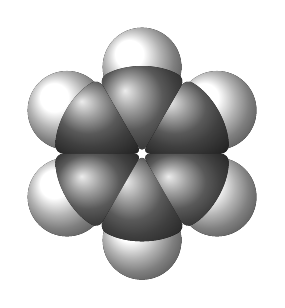
\begin{tikzpicture}[scale=1]
  \foreach \x in {30,90,150,210,270,330}
  {
    \fill[ball color=white](\x:1.1)circle(0.5);
    \fill[ball color=gray,rounded corners=3pt](0,0)--(\x-30:1.1)arc(\x-30:\x+30:1.1)--cycle;
  }
\end{tikzpicture}
\end{document}